\documentclass[12pt,xcolor=svgnames]{beamer}
\usepackage{dsfont,natbib,setspace}
\usepackage{tabularx}
\usepackage{accents}
\mode<presentation>

% replaces beamer foot with simple page number
\setbeamertemplate{navigation symbols}{}
\setbeamertemplate{footline}{
  \vspace{-1.5cm}
  \raisebox{10pt}{\makebox[\paperwidth]{\hfill\makebox[20pt]{\color{gray}\scriptsize\insertpagenumber}}}}

% colors
\newcommand{\bk}{\color{black}}
\newcommand{\rd}{\color{red}}
\newcommand{\fg}{\color{ForestGreen}}
\newcommand{\mar}{\color{Maroon}}
\newcommand{\org}{\color{Orange}}
\newcommand{\bl}{\color{blue}}
\newcommand{\gr}{\color{gray}}
\newcommand{\theme}{\color{FireBrick}}
\newcommand{\fb}{\color{FireBrick}}
\newcommand{\hlf}{\setstretch{1}}

% common math markups
\newcommand{\bs}[1]{\boldsymbol{#1}}
\newcommand{\mc}[1]{\mathcal{#1}}
\newcommand{\mr}[1]{\mathrm{#1}}
\newcommand{\bm}[1]{\mbox{\boldmath $#1$}}
\newcommand{\mb}[1]{\mathbf{#1}}
\newcommand{\ds}[1]{\mathds{#1}}

% spacing and style shorthan
\newcommand{\sk}{\vspace{.4cm}}
\newcommand{\nochap}{\vspace{0.5cm}}
\newcommand{\nsk}{\vspace{-.4cm}}
\newcommand{\chap}[1]{{\theme \Large \bf #1} \sk}
\newcommand{\R}[1]{{\bl\tt #1}}
\newcommand{\til}{{\footnotesize$\bs{\stackrel{\sim}{}}$ }}

% specific stats markups for this doc
\newcommand{\E}{\ds{E}}
\newcommand{\Reals}{\ds{R}}
\newcommand{\pr}{\text{Pr}}
\newcommand{\var}{\text{var}}
\newcommand{\cov}{\text{cov}}
\newcommand{\mT}{\mc{T}}
\newcommand{\GP}{\mc{GP}}
\newcommand{\iidsim}{\stackrel{\mathrm{iid}}{\sim}}
\newcommand{\indsim}{\stackrel{\mathrm{ind}}{\sim}}
\newcommand{\mN}{\mc{N}}
\newcommand{\mL}{\mc{L}}


\begin{document}

{ \usebackgroundtemplate{}%\includegraphics[height=\paperheight]{phoenix}}
\thispagestyle{empty}
\setcounter{page}{0}

%first review sampling distributions, then talk about sampling distributions for the OLS parameters, then prediction
%right now it goes prediction, review, OLS params, prediction

\title{\theme \Large \vskip 0.5cm
{\bf VectorBiTE Training 2018 \\ Methods Workshop}\\
\bigskip
\bf {\sf \gr Introduction to Bayesian Statistics}}

\author{
\begin{center}

\includegraphics[scale=0.15,trim=10 10 0 150]{VB_logo}
\end{center}
\texttt{\rd\small www.vectorbite.org}
%Normal distribution, distribution of the sample mean, \\
%Central Limit Theorem, Confidence Intervals
%and Method of Moments
%Review of sampling distributions
%Parameter estimation, sampling distributions,\\ 
%coefficient testing, and prediction intervals\\
%\vskip 1cm {\bf Leah R.~Johnson}\\ 
%{\org Virginia Tech}, Statistcs\\
%  \vskip .5cm \texttt{\rd\small leah.johnson-gramacy.com/QED/teaching}
}
\date{}
\maketitle 
}

% doc spacing
\setstretch{1.1}


\begin{frame}
\chap{Learning Objectives}

\begin{enumerate}
\item Understand the basic principles underlying Bayesian modeling methodology
\item  Introduce how to use Bayesian inference for real-world problems
\item Introduce computation tools to perform inference for simple models in R (how to turn the Bayesian crank)
\item Appreciate the need for sensitivity analysis, model checking and comparison, and the potential dangers of Bayesian methods.
\end{enumerate}

\end{frame}


\begin{frame}
\chap{Recall: Bayes Theorem} 

Bayes Theorem allows us to relate the conditional probabilities of two events $A$ and $B$:

\begin{equation*}
\pr(A|B) = \frac{\pr(B|A)\pr(A)}{\pr(B)}
\end{equation*}

\end{frame}

\begin{frame}
\chap{What is Bayesian Inference?} 

In the Bayesian approach our probabilities numerically represent rational beliefs. Bayes rule provides a rational method for updating those beliefs in light of new information and incorporating/quantifying uncertainty in those beliefs.\\

\sk

Thus, Bayesian inference is an approach for understanding data inductively. 

\end{frame}

\begin{frame}
\chap{What is Bayesian Inference?} 

We can re-write Bayes rule in terms of our parameters, $\theta$ and our data, $Y$:
\begin{align*}
\text{Pr}(\theta|Y) & = \frac{\text{Pr}(Y|\theta)\text{Pr}(\theta)}{\text{Pr}(Y)}\\
\end{align*}

The LHS is the main quantity of interest in a Bayesian analysis, the {\bl posterior},  denoted $f(\theta|Y)$:
\begin{equation*}
\overbrace{f(\theta|Y)}^\text{Posterior} \propto \overbrace{\mathcal{L}(\theta; Y)}^\text{Likelihood} \times \overbrace{f(\theta)}^\text{Prior}
\end{equation*}


\end{frame}


\begin{frame}
\chap{Bayesian methods provide} 

\begin{enumerate}
\item models for rational, quantitative learning
\item parameter estimates with good statistical properties
\item estimators that work for small and large sample sizes
\item parsimonious descriptions of data, predictions for missing data, and forecasts for future data
\item a coherent computational framework for model estimation, selection and validation
\end{enumerate}


\end{frame}



\begin{frame}
\chap{Classical vs Bayesian} 

The fundamental differences between classical and Bayesian methods is what is fixed and what is random in an analysis

\sk
\sk
\begin{center}
\begin{tabular}{|l|c|c|}
\hline
Paradigm & Fixed & Random \\
\hline
Classical & param ($\theta$) & data ($Y$)\\
\hline
Bayesian & data ($Y$) & param ($\theta$)\\
\hline
\end{tabular}
\end{center}
\end{frame}


\begin{frame}
\chap{Why/Why Not Bayesian Statistics?} 

{\footnotesize
{\bf \bl Pros}
\begin{enumerate}
\item If $f(\theta)$ \& $\mathcal{L}(\theta; Y)$ represent a rational person's beliefs, then Bayes' rule is an optimal method of updating these beliefs given new info (Cox 1946, 1961; Savage 1954; 1972).
\item Provides more intuitive answers in terms of the probability that parameters have particular values. 
\item In many complicated statistical problems there are no obvious non-Bayesian inference methods.
\end{enumerate}
{\bf \bl Cons}
\begin{enumerate}
\item It can be hard to mathematically formulate prior beliefs (choice of $f(\theta)$ often ad hoc or for computational reasons)
\item Posterior distributions can be sensitive to prior choice.
\item Analyses can be computationally costly.
\end{enumerate}
}

\end{frame}





\begin{frame}
\chap{Steps to Making Inference} 


\begin{enumerate}
\item Research question
\item Data collection
\item Model $Y_i \approx f(X_i)$ 
\item Estimate the parameter in the model with uncertainty
\item Make inference
\end{enumerate}

The difference between {\bl Classical} and {\bl Bayesian} lies in step 4: (C) uses maximum likelihood estimate (MLE), and (B) derives a posterior distribution.
\end{frame}


\begin{frame}
\chap{Example: Estimating the probability of a rare event}

Suppose we are interested in the prevalence of an infectious disease in a small city.  A small random sample of 20 individuals will be checked for infection.
\begin{itemize}
\item Interest is in the fraction of infected individuals
\begin{align*}
\theta \in \Theta =[0,1]
\end{align*}
\item The data records the number of infected individuals
\begin{align*}
y \in \mathcal{Y} =\{0,1, \ldots, 20\}
\end{align*}
\end{itemize}

\end{frame}

\begin{frame}
\chap{Example: Likelihood/sampling model}

Before the sample is obtained, the number of infected individuals is unknown. 
\begin{itemize}
\item Let $Y$ denote this to-be-determined value
\item If $\theta$ were known, a sensible {\bl sampling} model is
\begin{align*}
Y|\theta \sim \mr{Bin} (20, \theta)
\end{align*}
\end{itemize}
\begin{center}
\includegraphics[scale=0.375,trim=20 50 0 100]{bin_sampling}
\end{center}

\end{frame}


\begin{frame}
\chap{Example: Prior}

Other studies from various parts of the country indicate that the infection rate ranges from about
0.05 to 0.20, with an average prevalence of 0.1. 
\begin{itemize}
\item Moment matching from a beta distribution (a convenient choice) gives the prior
\begin{align*}
\theta \sim \mr{Beta} (2,20)
\end{align*}
\end{itemize}
\begin{center}
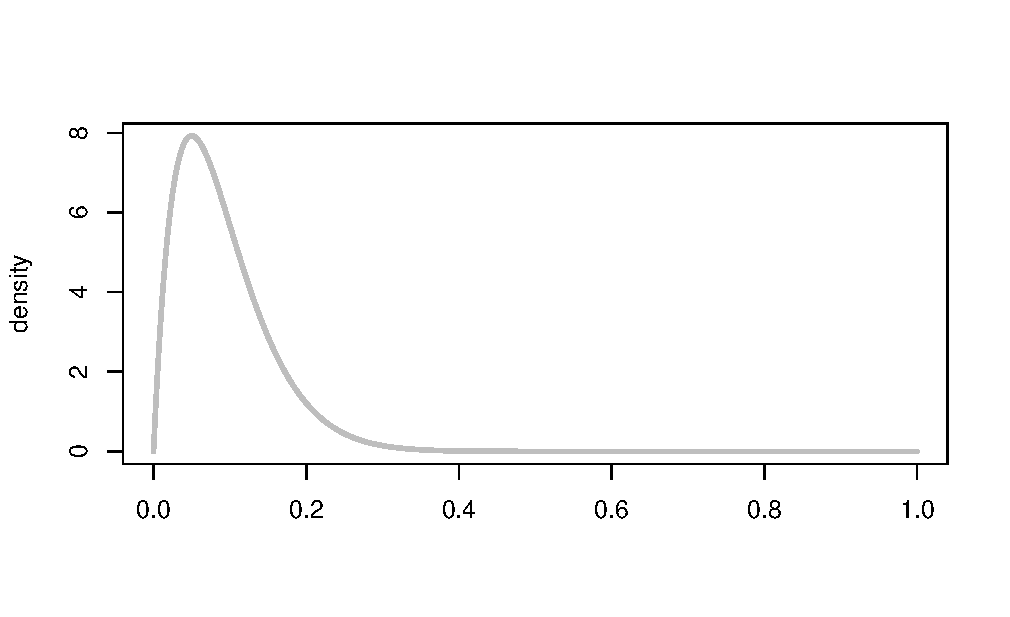
\includegraphics[scale=0.55,trim=10 50 0 125]{beta_prior}
\end{center}

\end{frame}


\begin{frame}
\chap{Example: Posterior}

The prior and sample model combination:
\begin{align*}
\theta & \sim \mr{Beta} (a,b)\\
Y|\theta &  \sim \mr{Bin} (n, \theta)
\end{align*}
and an observed $y$ (the data), leads to the posterior 
\begin{align*}
p(\theta|y)=\mr{Beta}(a+y, b+n-y)
\end{align*}

\end{frame}


\begin{frame}
\chap{Example: Posterior}

For our case, we have $a=2$, $b=20$, $n=20$. \\

If we don't find any infections, then $y=0$ our posterior is:
\begin{align*}
p(\theta|y=0)=\mr{Beta}(2, 40)
\end{align*}
\begin{center}
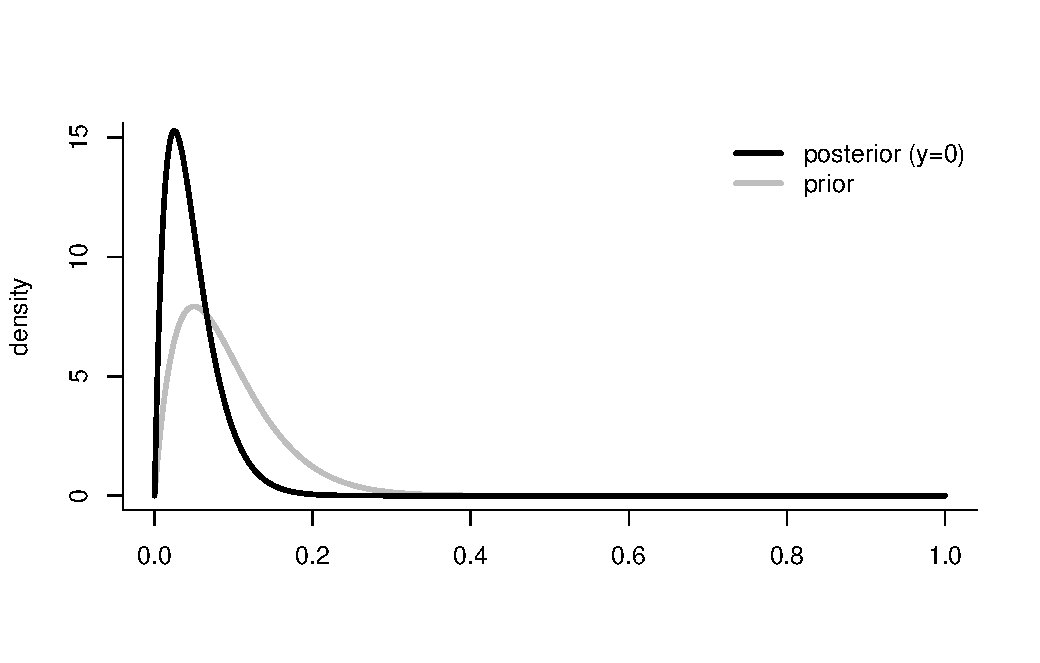
\includegraphics[scale=0.55,trim=10 50 0 60]{beta_bin_posterior}
\end{center}

\end{frame}

\begin{frame}
\chap{Example: Sensitivity Analysis }

How influential is our prior?

The posterior expectation is
\begin{align*}
\mr{E}\{\theta|Y=y\} =   \frac{n}{w+n} \bar{y} + \frac{w}{w+n} \theta_0
\end{align*}
a weighted average of the sample mean and the prior expectation:
\begin{align*}
\theta_0 & =  \frac{a}{a+b} ~~~~ {\rd \rightarrow} \text{ prior expectation (or guess)}\\
w & = a + b  ~~~~ {\rd \rightarrow} \text{  prior confidence} 
\end{align*}


\end{frame}


\begin{frame}
\chap{Example: A non-Bayesian approach}

A standard estimate of a population proportion, $\theta$ is the sample mean  $\bar{y} = y/n$, the fraction of infected people in the sample. 

\sk
If $y=0$, this gives zero, so reporting the sampling uncertainty is crucial (e.g., for reporting to health officials). 

\sk
The most popular 95\% confidence interval for a population proportion is the {\bl Wald Interval}:
\begin{equation*}
\bar{y} \pm 1.96 \sqrt{\bar{y}(1-\bar{y})/n}.
\end{equation*}
This has the correct {\it asymptotic} coverage, but {\rd $y=0$ is still problematic}!

\end{frame}


\begin{frame}
\nochap
{\bf \fb Exercise: is a treatment for cancer effective?}\\

{\footnotesize
We have data on $n$ cancer patients that have been given a particular treatment. Our outcome variable is whether or not it was ``effective'':
\begin{center}
 \begin{tabular}{lll}
Patient & Effectiveness & Numerical Data \\
1& N& 0\\
2&N&0\\
3&Y&1\\
\vdots &\vdots &\vdots \\
\end{tabular}
\end{center}
The appropriate sampling model for each patient is a Bernoilli:
$$Y_i|\theta  \stackrel{iid}{\sim} f(Y|\theta) = \text{Bern}(\theta)$$ 
where $\theta$ is the success rate of the treatment. Based on this, write down the likelihood for the $n$ patients. Then, assuming a $\mr{Beta}(a,b)$ prior for $\theta$ find the posterior distribution for $\theta|Y$. Does this look familiar?
}

\end{frame}


\iffalse
\begin{frame}
\begin{enumerate}



\item[4. ] {\bf Posterior:}
First we need to decide on an appropriate  {\bl prior} for $\rho.$ To look at the domain of $\rho$ we recall that 
\begin{equation*}
\rho = \pr(Y_i = 1),\Rightarrow \rho \in [0, 1] 
\end{equation*}
Hence, either a {\bl Beta} or a {\bl Uniform} distribution can be a prior for $\rho.$ Say we chose $\text{Beta}(a,b)$ with $a$ and $b$ specified as $a=b=1$ or $a=1,b=3$. Thus,

$$ f(\rho) = \text{Beta}(a,b).$$
\end{enumerate}
\end{frame}

\begin{frame}
\begin{enumerate}

\item[4. ] {\bf Posterior: continued} 

Next, we need to derive the likelihood. We have $Y_i|\rho   \stackrel{iid}{\sim} f(Y|\rho) = \text{Bern}(\rho),$ where $Y_i|\rho$ are assumed to be {\bl conditionally} independent and identically distributed, thus the likelihood is given by

\begin{align*}
f(\tilde{Y}|\rho) &= f(Y_1, Y_2, \cdots Y_5|\rho)\\
& \stackrel{iid}{=}  f(Y_1|\rho) f(Y_2|\rho)  \cdots f(Y_5|\rho)\\
& = \prod_{i=1}^{n=5} f(Y_i|\rho).
\end{align*}
\end{enumerate}
\end{frame}


\begin{frame}
\begin{enumerate}

\item[4. ] {\bf Posterior: continued} 

Now we can use {\bl Bayes} formula to calculate the posterior distribution as follows
\begin{align*}
f(\rho|\tilde{Y}) &\propto \prod_{i=1}^{n=5} f(Y_i|\rho) f(\rho)\\
&\propto  \prod_{i=1}^{n=5} \text{Bern}(Y_i|\rho)\text{Beta}(a,b)\\
&\propto  \prod_{i=1}^{n=5} \rho^{Y_i} (1- \rho)^{n-Y_i} \dfrac{\Gamma (a+b)}{\Gamma (a)\Gamma (b)} \rho^{a-1} (1-\rho)^{b-1}
\end{align*}

Does this look like a known distribution? What do we do?

\end{enumerate}
\end{frame}


\begin{frame}
\begin{enumerate}

\item[4. ] {\bf Posterior: continued} 

We play the game {\bl name that distribution}
\begin{enumerate}
\item[a.] Simplify the best you can
\item[b.] $\ast$ , $\div$ by constants
\item[c.] Remember what is the RV in the expression
\item[d.] Look for {\bl Kernels} of known distributions
\end{enumerate}
\sk
{\rd Definition:} The {\bl Kernel} of a probability density function (or mass function) are all components which include the random variable. 

eg: Let $Y_i \sim \textbf{N}(\mu, \sigma^2),$ with random variable $\mu$

$$ f(Y_i) = \underbrace{\dfrac{1}{\sqrt{2\pi \sigma^2}}}_{constant} \underbrace{e^{-\dfrac{1}{2\sigma^2}(Y_i - \mu)^2}}_{Kernel}$$ 
\end{enumerate}
\end{frame}


\begin{frame}
\begin{enumerate}

\item[4. ] {\bf Posterior: continued} 

Back to our example: 
\begin{align*}
f(\rho|\tilde{Y}) &\propto  \prod_{i=1}^{n=5} \rho^{Y_i} (1- \rho)^{n-Y_i} \dfrac{\Gamma (a+b)}{\Gamma (a)\Gamma (b)} \rho^{a-1} (1-\rho)^{b-1}\\
&\propto \rho^{\sum Y_i} (1- \rho)^{n-\sum Y_i} \dfrac{\Gamma (a+b)}{\Gamma (a)\Gamma (b)} \rho^{a-1} (1-\rho)^{b-1}\\
&\propto \rho^{\sum Y_i +a -1} (1- \rho)^{n-\sum Y_i +b -1} \\
&\propto \textbf{Beta} \left(\underbrace{\sum Y_i +a}_{a^*}, \underbrace{n-\sum Y_i +b}_{b^*}\right),
\end{align*}
where
$ \textbf{Beta}(a^*, b^*) = \dfrac{\Gamma (a^*+b^*)}{\Gamma (a^*)\Gamma (b^*)} \rho^{a^*-1} (1-\rho)^{b^*-1}.$

{\rd Now what do we do with this posterior?}

\end{enumerate}
\end{frame}





\begin{frame}
\begin{enumerate}

\item[5.] {\bf Make inference:} We summarize the posterior to make inference using the following statistics
\begin{enumerate}
\item[a.] Expectation $\text{E}(\rho|\tilde{Y})$% = \dfrac{a^*}{a^* +b^*} = 0.25$
\item[b.] Maximum A Posteriori (MAP) $\text(Mode) (f(\rho|\tilde{Y})$% = = \dfrac{a^* -1}{a^* +b^* -2} = 0.2$
\item[c.] Variance $\text{Var}(\rho|\tilde{Y} )$%= (.12)^2$
\item[d.] Calculate $\pr(\rho<.5|\tilde{Y}) $%= .96$
\item[e.] Q Credible Interval $\pr(\rho \in [L, U] |\tilde{Y}) = Q,$ with $L = \dfrac{1-Q}{2},$ and $U = \dfrac{1-Q}{2} +Q$
\item[f.] Q Highest Posterior Density Interval (HPDI) $\pr(\rho \in [L, U] |\tilde{Y}) = Q,$ where $L$ and $U$ are chosen so that $U-L$ is the shortest
\end{enumerate}
 \end{enumerate}
\end{frame}


\begin{frame}
\begin{enumerate}

\item[5.] {\bf Inference Statements} 

{\bf For a, b, c:} Given the data, we predict that the probability that the cancer drug is effective is $\text{E}(\rho|\tilde{Y})$ or  $\text{MAP}(\rho|\tilde{Y})$ with variance $\text{Var}(\rho|\tilde{Y})$. \\

{\bf For d:} Given the data, we infer the prob of the cancer drug being effective is low because $\pr(\rho<.5|\tilde{Y}) = .96$ or high because $\pr(\rho<.5|\tilde{Y}) = .2$\\

{\bf For e, f:} Given the data, the probability that $\rho \in [L, U]$ is Q. \\

{\rd \bf Note:} {\bf QCI} Describes the behavior of the {\bl  tail} of the posterior distribution and { \bf HPDI} Describes where the {\bl mean} of the posterior distribution is.\\


\end{enumerate}
\end{frame}

\fi

\begin{frame}
\chap{Conjugate Bayesian Models}

Some sets of priors/likelihoods/posteriors exhibit a special relationship called {\em \bl conjugacy}. This happens if the posterior distribution has the same form as the prior. For instance, in our above Beta-Binomial/Bernoilli examples:
\begin{align*}
\theta & \sim \mr{Beta} (a,b)\\
Y|\theta &  \sim \mr{Bin} (n, \theta)\\
\theta | Y & \sim \mr{Beta}(a*, b*)
\end{align*}
{\em Are all posteriors in the same family as the priors?} {\rd \bf No}\\

Conjugacy is a nice special property, but most of the time this isn't the case and getting an analytic form of the posterior distribution can be hard or impossible.  

\end{frame}

\begin{frame}
\chap{What do you do with a Posterior?}


\end{frame}



\end{document}